\chapter{Introduction}\label{ch:intro}

\section{The Nuclear Fuel Cycle}

The nuclear fuel cycle, in general, can be described as a set of facilities that
interact with one another to either provide or consume fuel services. The
overall goal of the nuclear fuel cycle is to provide fuel to nuclear power
plants which, in turn, generate energy. The overall goal of the system is to
produce power at a competitive price while managing externalities of the
process, the chief of which is spent nuclear fuel. There exist a myriad of
strategies to achieve this aim which generally fall along a spectrum of the
degree to which fuel is recycled. In general, fuel cycles on the end of the
spectrum that does not recycle fuel are concerned most with cost, whereas fuel
cycles that fully recycle fuel are concerned most with issues of sustainability
and intergenerational equity.

\subsection{The Open Fuel Cycle}
The open, or once-through, fuel cycle is relatively simple and is in place in
most countries in the world that currently utilize nuclear power. In practice,
the primary fuel element used in this type of cycle is uranium; however,
processed fertile material, such as thorium, can also be used. The fuel cycle is
considered open because fuel that is used in a reactor is stored indefinitely
once its reactivity has dropped below useful levels.

Beginning the fuel cycle process, uranium ore is initially extracted from the
ground using one of a variety of techniques including open pit mining,
underground mining, and \textit{in situ} leaching. The uranium ore is then
milled to form yellowcake, $\mathrm{U_3O_8}$. The tailings, or byproducts, of
this process are slightly radioactive and are therefore considered to be
low-level waste (LLW) by the Nuclear Regulatory Commission (NRC)
(see \cite{nrc_10_1985}).

Certain reactors are designed to use naturally enriched uranium. For these
reactors, yellowcake can be directly reduced with oxygen to form naturally
enriched uranium oxide, $\mathrm{UO_2}$. For the majority of power reactors,
however, the uranium must be enriched with higher-than-natural levels of
uranium-235. In order to do so, yellowcake is sent to a conversion facility,
which converts it from $\mathrm{U_3O_8}$ to $\mathrm{UF_6}$. The uranium
hexafluoride is then enriched to the required level in an enrichment facility,
of which three classes exist: gaseous diffusion, the original enrichment
technology; centrifugal diffusion, the current enrichment technology; and Atomic
Vapor Laser Isotope Separation (AVLIS), a newer technology not currently in
commercial production. The enriched uranium hexafluoride is then sent to a fuel
fabrication facility where it is returned to yellowcake form before being
reduced to uranium oxide. The uranium oxide is then sintered into pellets and
loaded into fuel assemblies to be placed in a reactor. This process, in
conjunction with uranium mining, is termed the \textit{front end} of the nuclear
fuel cycle.

Once fuel has been processed in a reactor, it is cooled off in pools for a
number of years, and then stored in dry casks before eventually being sent to a
final repository. The physical location of the fuel may vary during dry cask
storage between the reactor site or some other interim storage site.

Graphically, the open fuel cycle is shown in Figure \ref{fig:open-cycle}.

\begin{figure}[]
  \begin{center}
    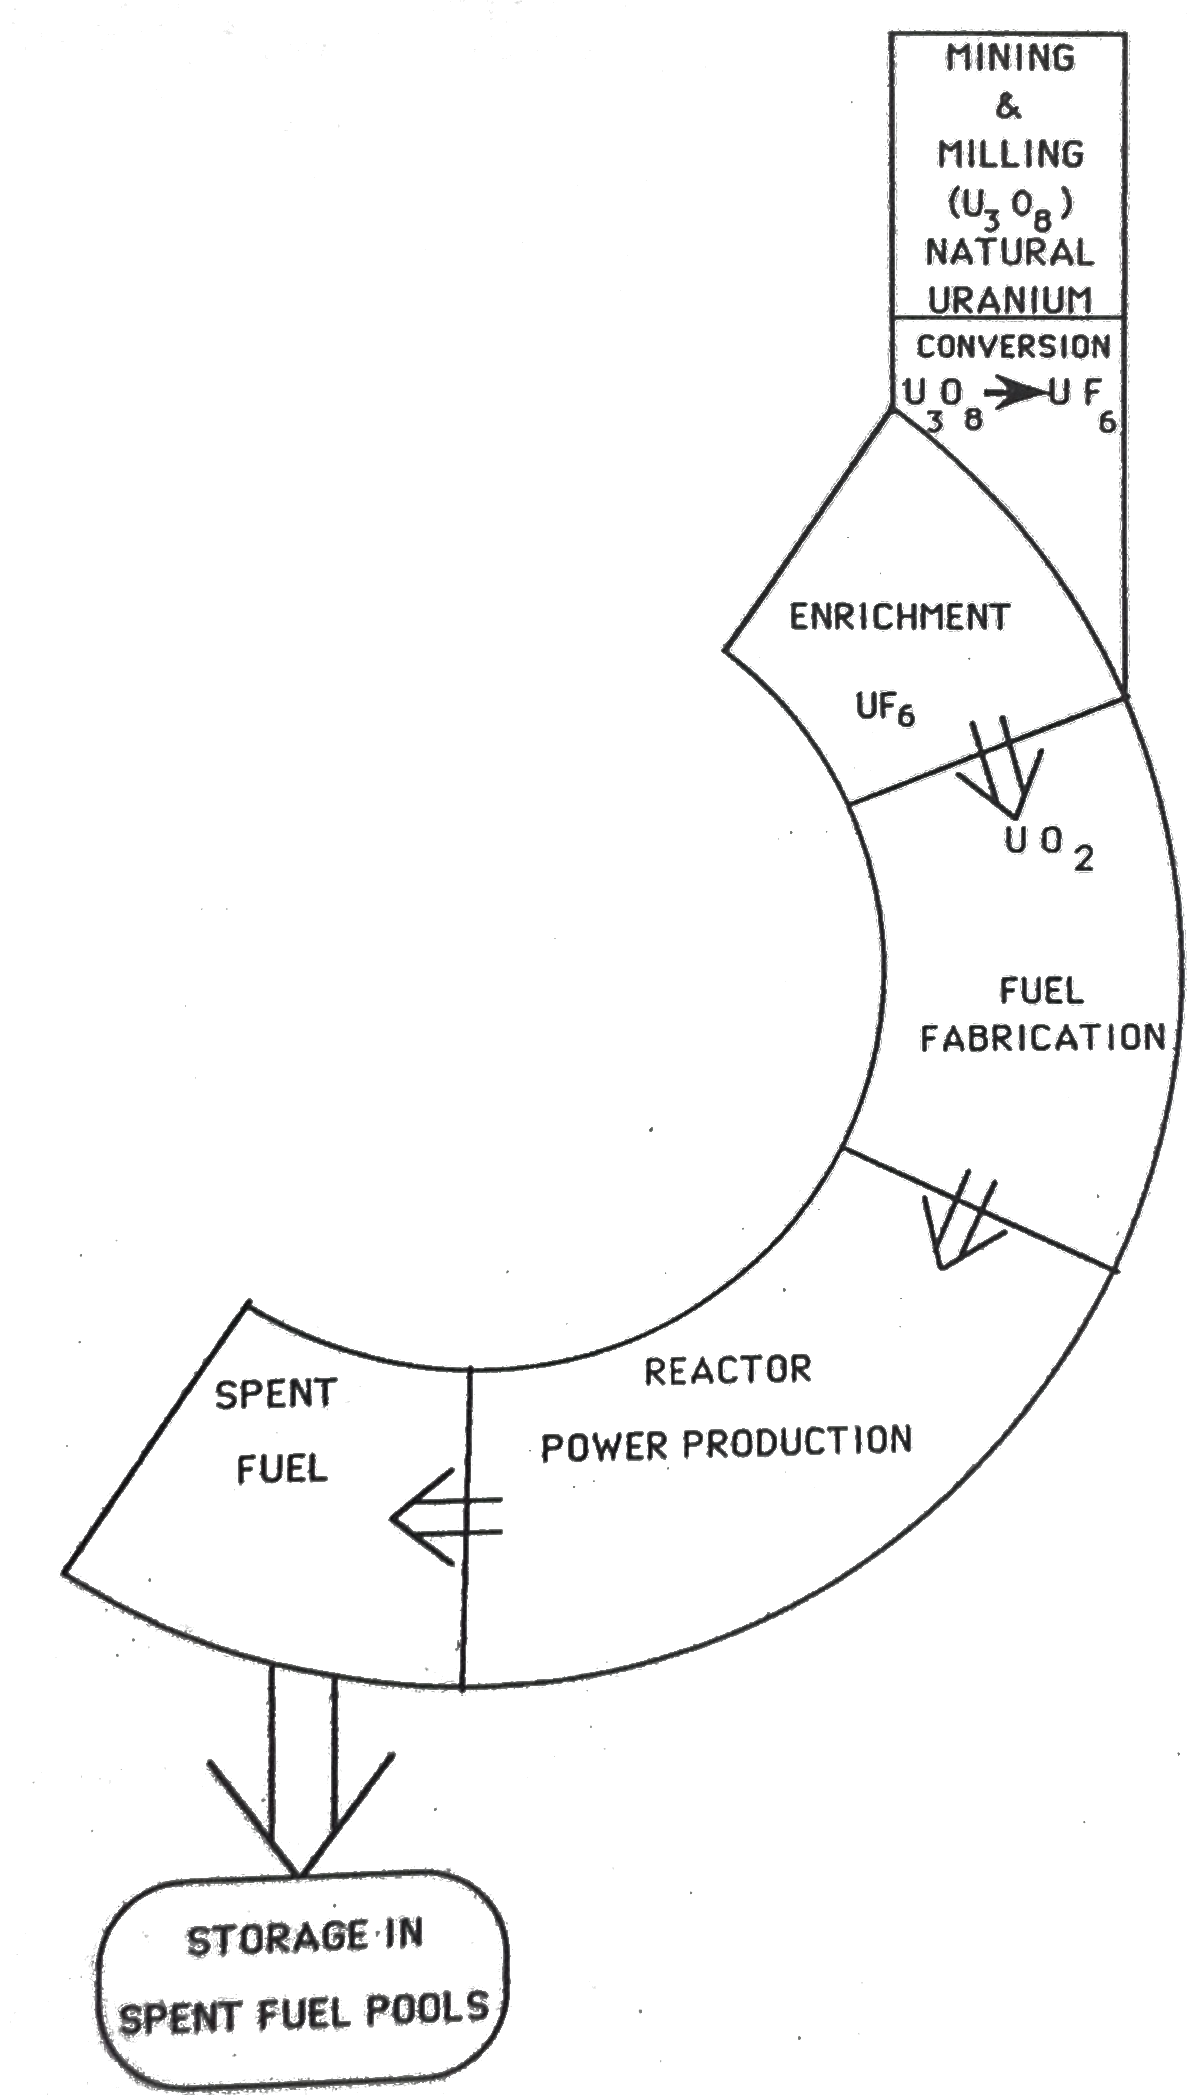
\includegraphics[height=7.5cm]{./chapters/intro/open_cycle.png}
  \caption{The once-through fuel cycle as shown in \cite{cochran1990nuclear}.}
  \label{fig:open-cycle}
  \end{center}
\end{figure}


\subsection{The Modified-Open Fuel Cycle}

\subsection{The Closed Fuel Cycle}

\section{Fuel Cycle Simulation}

\subsection{Simulator Classification}

\subsection{Metrics}

\subsection{Benchmarks}

\section{Open Questions in Fuel Cycle Simulation}

\subsection{Using Agent-Based Models}

\subsection{Input Fuel Isotopic Matching}

\subsection{Modeling Global Regions}
